\documentclass{bmcart}

%%%%%%%%%%%%%%%%%%%%%%%%%%%%%%%%%%%%%%%%%%%%%%
%%                                          %%
%% CARGA DE PAQUETES DE LATEX               %%
%%                                          %%
%%%%%%%%%%%%%%%%%%%%%%%%%%%%%%%%%%%%%%%%%%%%%%

%%% Load packages
\usepackage{amsthm,amsmath}
\usepackage{graphicx}
%\RequirePackage[numbers]{natbib}
%\RequirePackage{hyperref}
\usepackage[utf8]{inputenc} %unicode support
%\usepackage[applemac]{inputenc} %applemac support if unicode package fails
%\usepackage[latin1]{inputenc} %UNIX support if unicode package fails
\usepackage[spanish]{babel}


%%%%%%%%%%%%%%%%%%%%%%%%%%%%%%%%%%%%%%%%%%%%%%
%%                                          %%
%% COMIENZO DEL DOCUMENTO                   %%
%%                                          %%
%%%%%%%%%%%%%%%%%%%%%%%%%%%%%%%%%%%%%%%%%%%%%%

\begin{document}

	\begin{frontmatter}
	
		\begin{fmbox}
			\dochead{Research}
			
			%%%%%%%%%%%%%%%%%%%%%%%%%%%%%%%%%%%%%%%%%%%%%%
			%% INTRODUCIR TITULO PROYECTO               %%
			%%%%%%%%%%%%%%%%%%%%%%%%%%%%%%%%%%%%%%%%%%%%%%
			
			\title{Tiroiditis}
			
			%%%%%%%%%%%%%%%%%%%%%%%%%%%%%%%%%%%%%%%%%%%%%%
			%% AUTORES. METER UNA ENTRADA AUTHOR        %%
			%% POR PERSONA                              %%
			%%%%%%%%%%%%%%%%%%%%%%%%%%%%%%%%%%%%%%%%%%%%%%
			
			\author[
			  addressref={aff1},                   % ESTA LINEA SE COPIA IGUAL PARA CADA AUTOR
			  corref={aff1},                       % ESTA LINEA SOLO DEBE TENERLA EL COORDINADOR DEL GRUPO
			  email={jane.e.doe@cambridge.co.uk}   % VUESTRO CORREO ACTIVO
			]{\inits{A.D}\fnm{Alejandro} \snm{Domínguez Recio}} % inits: INICIALES DE AUTOR, fnm: NOMBRE DE AUTOR, snm: APELLIDOS DE AUTOR
		
			\author[
			  addressref={aff1},                   % ESTA LINEA SE COPIA IGUAL PARA CADA AUTOR
			  email={rafatravil@gmail.com}   % VUESTRO CORREO ACTIVO
			]{\inits{R.T}\fnm{Rafael} \snm{Trapero Vílchez}} % inits: INICIALES DE AUTOR, fnm: NOMBRE DE AUTOR, snm: APELLIDOS DE AUTOR
		
			
			%%%%%%%%%%%%%%%%%%%%%%%%%%%%%%%%%%%%%%%%%%%%%%
			%% AFILIACION. NO TOCAR                     %%
			%%%%%%%%%%%%%%%%%%%%%%%%%%%%%%%%%%%%%%%%%%%%%%
			
			\address[id=aff1]{%                           % unique id
			  \orgdiv{ETSI Informática},             % department, if any
			  \orgname{Universidad de Málaga},          % university, etc
			  \city{Málaga},                              % city
			  \cny{España}                                    % country
			}
		
		\end{fmbox}% comment this for two column layout
		
		\begin{abstractbox}
		
			\begin{abstract} % abstract
			
			%%%%%%%%%%%%%%%%%%%%%%%%%%%%%%%%%%%%%%%%%%%%%%%
			%% RESUMEN BREVE DE NO MAS DE 100 PALABRAS   %%
			%%%%%%%%%%%%%%%%%%%%%%%%%%%%%%%%%%%%%%%%%%%%%%%	
			
			\end{abstract}
			
			%%%%%%%%%%%%%%%%%%%%%%%%%%%%%%%%%%%%%%%%%%%%%%
			%% PALABRAS CLAVE DEL PROYECTO              %%
			%%%%%%%%%%%%%%%%%%%%%%%%%%%%%%%%%%%%%%%%%%%%%%
			
			\begin{keyword}
			\kwd{sample}
			\kwd{article}
			\kwd{author}
			\end{keyword}
		
		
		\end{abstractbox}
	
	\end{frontmatter}
	

	\section{Introducción}

\hrule
\vspace{5mm}
\\
La tiroides es una glándula pequeña situada en la parte anterior del cuello, encargada de la producción de dos hormonas tiroideas: la tiroxina (T4), que 
corresponde al 93 por ciento de hormona secretada por la glándula tiroides, y la 3,5,3-triyodotironina (T3) \cite{Stegmann} . Esta regula procesos metabólicos esenciales tanto en la etapa de desarrollo como en la edad adulta. \cite{Stegmann} 
\\ \\
El término tiroiditis (HP:0100646) se asocia con todas aquellas enfermedades que presenten inflamación de la glándula tiroides \cite{Sweeney2014}. Los síntomas que produce la tiroiditis variarán dependiendo de la enfermedad tiroidea que la produzca. No obstante, podemos diferenciar dos efectos diferenciados provocados por la tiroiditis \cite{Pulgarin} : 
\begin{itemize}
    \item Hipotiroidismo. Condición en la cual la glándula tiroides no puede producir la suficiente cantidad de hormonas tiroideas necesarias para cumplir con el requerimiento tisular.
    \item Hipertiroidismo. Incremento sostenido de las hormonas tiroideas debido al aumento de biosíntesis y secreción de la tiroides.
\end{itemize} 
\\ \\
Entre las enfermedades más conocidas que presenten tiroiditis tenemos la enfermedad de Hashimoto (HT). Es conocido que alredeor del 20-30 por ciento de la población sufre de HT. \cite{Zheng2020}. Principalmente la sintomatologia de HT es bocio-no doloroso, hipotiroidismo y elevación de TPO \cite{Sweeney2014}. A su vez existen otros subtipos tales como tiroiditis infecciosa, tiroiditis post-parto o tiroiditis inducida por radiación. \cite{Sweeney2014}
\\ \\
 Diversos factores  intervienen en el desarrollo de estas enfermerdades, como por ejemplo los factores de tipo ambiental (infecciones producidas por agentes externos), factores dietéticos (relacionados con los niveles de ingesta de yodo) u otro tipo de factores como el estrés, el tabaquismo o incluso el embarazo. \cite{Hiromatsu}
\\  \\ 
 Por ejemplo, hablando de la enfermedad de Hashimoto, el 50 por ciento de los factores que producen dicha enfermedad son genéticos, por lo que nos encontramos ante aquellos factores de mayor implicación. Siendo la característica más común, una elevación de los anticuerpos autoinmunes TPOAb y TGAb en las celulas tiroideas.\cite{Zheng2020} A su vez se ha encontrado una alta coexistencia de HT con la diabetes tipo 1, Turner syndrome, Addison disease, and  hepatitis C no tratada.\cite{Sweeney2014}
\\ \newpage
Hasta la fecha varios genes se han asociado al fenotipo, como el HLA-DR, los genes inmunorreguladores (CD40, CTLA-4, PTPN22, FOXP3 y CD25) y genes específicos del tiroides (tiroglobulina [TG] y receptor de la hormona tiroestimulante [TSH]), siendo estos son los más citados; no obstante, encontramos un total de 46 genes asociados al fenotipo. 
\\ \\
Estos genes principalmene están relacionados con dos procesos moleculares: la unión de proteínas y péptidos (importante en la estructura del cromosoma) y en la actividad de los receptores inmunes. Dicha actividad consiste en recibir señales y transmitirlas a células para iniciar una respuesta inmune en éstas.
\cite{Hiromatsu}
En la actividad de los receptores inmunes, están implicados los genes IL2RG, IL7R, IL2RA, HLA-DQB1 y HLA-DQA1. Podemos destacar estos dos últimos, siendo ambos pertenecientes a la clase MHC (Major histocompatibility complex). Ambos genes juegan un papel fundamental en el sistema inmune ya que presentan aquellos péptidos de proteínas extracelulares. \cite{HLA} 
\\ \\
Sin embargo,los genes restantes no se encargan de la unión de proteínas, pues encontramos varios que no participan en ninguno de los dos procesos moleculares. Destacar que  la familia de ILR, compuesta por IL2RG, IL7R y IL2RA , participan en ambos procesos, por lo que podemos afirmar que son de gran importancia en la tiroiditis. 

En la siguiente imagen podemos ver la red de genes relacionados con nuestro fenotipo, siendo representados de azul aquellos que intervienen en la actividad de los receptores inmunes, de rojo los que intervienen en la unión de péptidos y bicolor los que intervienen en ambas.
\begin{center}
 
    \includegraphics[scale=0.4]{figures/red de genes.png}
    
    Figure 2.1. Red de Genes
\end{center}
\\ \\
Dada la importancia de los factores genéticos en este fenotipo (HP:0100646), el estudio se centrará en la realización de un análisis de los diferentes genes asociados a dicho fenotipo y de las relaciones funcionales entre estos. 
\\ \\  \newpage 
Se tendrán en cuenta el tipo de interacción (física, co-expresión, databases, etc...) a partir de las cuales diluciar los diferentes clusters. Estos clusters ayudarán a clasificar genes en base a la función molecular que desempeñen. La distribución de genes resultante ayudará a descubrir cuales de ellos tienen una mayor relevancia.
\\ \\





	\newpage
\section{Materiales y métodos}

Con todas las herramientas y materiales  que se exponen a continuación se ha realizado el  estudio. Se ha seguido el flujo de trabajo que se muestra en la imagen siguiente:

\begin{center}
 
    \includegraphics[scale=0.5]{figures/Diagrama sin título.drawio.png}
    
    Figure 2.1. Flujo de trabajo
\end{center}


\subsection*{Datos fenotipos}
El paso inicial fue descargar los datos genotípicos sobre los dos fenotipos a estudiar (HP:0100646 Thyroiditis y HP:0000872 Hashimoto) de la página web HPO (https://hpo.jax.org/app/).  HPO (The Human Phenotype Ontology) es un proyecto que ofrece la ontología de distintos tipos de fenotipos relevantes. Sus funciones son muy variadas; yendo desde su utilidad para dar diagnósticos médicos hasta para el uso de análisis bioinformáticos, como es el caso.
El conjunto inicial de interacciones gen-gen asociados a dichos fenotipos ha sido  obtenido a partir de la base de datos STRING (https://string-db.org/). La base de datos STRING integra conocimiento sobre las relaciones entre proteínas y genes, incluyendo desde interacciones físicas hasta relaciones funcionales. Las relaciones son determinadas a partir de una serie de evidencias con una significancia asociada. \cite{Szklarczyk2021}  Las evidencias que han determinado las redes de interacción de nuestros fenotipos son las siguientes: (1) textmining, (2) experimentos, (3) bases de datos, (4) co-expresión, (5) vecindad, (6) fusión de genes, (7) co-ocurrencia. La significancia mínima asociada a cada interacción determinada ha sido de 0.7. Finalmente, hemos encontrado un total de 46 genes asociados al fenotipo  HP: 0100646 (Thyroiditis) y 17 a  HP:0000872 (Hashimoto). 

\subsection*{Propagación de red}
Se realizó una propagación de red a los conjuntos de genes inciales (uno por cada fenotipo); obteniendo un total de 200 genes por conjunto (tal y como recomienda la literatura).\cite{Ghiassian2015} Para ello hemos usado la herramienta 'DIAMOnD' (DIseAse MOdule Detection). Esta herramienta identifica módulos que comparten 	
patrones de conectividad con el fin de determinar la principal propiedad topológica que los define, para su posterior extensión. \cite{Ghiassian2015} Se basa en algoritmos de deteccion de comunidades. Para dicha detección son usados tres métodos:
    \begin{itemize}
        \item Algoritmos de link community. Basados en similitudes de enlace entre los nodos. \cite{Ahn2010}
        \item Louvain method. Maximiza la funcion de modularidad global.\cite{Sanyal2006} 
        \item Markov Cluster Algorithm (MCL). Detecta regiones densas bansandose en un flujo aleatorio. \cite{MCL}
    \end{itemize}

Una vez detectadas todas las comunidades, éstas son evaluadas seleccionándose aquellas con una signifancia relevante (aquellas con un pvalor menor de 0.05 en el test de Fisher) \cite{Jafari2018}. El procedimiento sería el siguiente:
    \begin{itemize}
        \item La significancia de conectividad es determinada para todas los genes conectados a alguno de las comunidades detectadas.
        \item Los genes son clasificados en función de sus p-valores.
        \item Los genes con el menos p-valor se añaden a la semilla de nodos.
        \item Los pasos 1-3 se repiten añadiendo genes a las comunidades de uno en uno.
    \end{itemize}

\subsection*{LinkCommunities}
Se efectuó una búsqueda de  las comunidades presentes en ambas redes. Para dicha búsqueda usamos el paquete R 'linkcomm V1.0-11'. Linkcomm provee un conjunto de herramientas para generar, visualizar y analizar link communities en redes de tamaño y tipo arbitrario.  \cite{Kalinka2011} Se basa en un algoritmo que agrupa  los enlaces entre nodos en lugar de  agrupar los propios nodos.Esto permite que cada nodo pertenezca a múltiples comunidades, superpuestas o anidadas. \cite{Kalinka2011} 
\\
Uno de los parámetros a tener en cuenta es el threshold, el cual hace referencia a la altura a la que el dendograma es cortado. En función de este umbral, se obtienen mayor o menor número de clusters. Para este proyecto hemos optado por un threshold de 400, el cual no es demasiado restrictivo.



\subsection*{Enriquecimiento funcional}
El enriquecimiento funcional es crucial en la interpretación de datos ómicos. Este fue realizado, mediante análisis de sobrerrepresentación, a las comunidades presentes en las redes asociadas a cada fenotipo. El análisis de sobrerrepresentación es útil para determinar las funciones moleculares asociadas a un conjunto de genes. Este se encarga de determinar los procesos sobrerrepresentados (enriquecidos) dentro de un conjunto de genes mediante el test hipergeométrico. Analiza cada término KEGG, de forma aislada sin tener en cuenta la estructura de la jerarquía de términos. \cite{Zhang2010}

\\
Para su implementación se usó el paquete de R 'clusterProfiler 3.16'. Clusterprofiler fue diseñado para realizar análisis de sobrerepresentación usando términos GO y KEGG, entre otros. Actualmente soporta varias ontologías y anotaciones de pathways, y tiene miles de especies con capacidad de anotación. 
\\
Seleccionamos la ontología 'KEGG latest release 104', que  hace referencia a la Kyoto Enciclopedia de Genes y Genomas, una de las bases de datos biológicas más importantes actualmente. El mayor componente de información se denomina PATHWAY y consiste en diagramas asociados a rutas moleculares, incluyendo rutas metabólicas y regulativas. 
Se asignó a cada comunidad el pathway biólogico correspondiente en base al gene ratio obtenido tras el enriquecimiento.  El umbral del p-value ha sido fijado  en 0.05 para seleccionar solo aquellas comunidades más fieles a las distribución, tal y como se recomienda en la literatura.\cite{Jafari2018} \\  A la hora de filtrar aquellos pathways más significativos, se seleccionó también como umbral un gene ratio mayor o igual a 0.7. Para este filtrado solo tuvimos en cuenta el gene ratio de Tiroiditis.El de Hashimoto interesa que se bajo pues lo que se busca es aumentar la red de genes de dicho fenotipo.
 


	\newpage
\section{Resultados}

\subsection*{HPO}
Se encontraron un total de, 45 y 17 genes asociados a los fenotipos tiroiditis (HP:0100646) y Hashimoto (HP:000087) respectivamente.
\subsection*{String}
La red de interacciones obtenida a partir de los 45 genes asociados al fenotipo tiroiditis (HP:0100646), está formada por un total del 122 relaciones, con un grado medio en sus nodos de 5.42 y un coeficiente local de clustering de 0.539 (figura 3.1). Los procesos biológicos (BP, Gene Ontology), funciones moleculares (MF, Gene Ontology) o pathways (P, KEGG) con mejores resultados de anotación (Strenght Log10(observed / expected)) son: (BP, Gene Ontology) Inosine biosynthetic process, (MF, Gene Ontology) Immune receptor activity y (P, KEGG) Non-homologous end-joining , Strenght 2.46, 1.22 y 1.86 respectivamente \cite{StringHP:0100646} \\ \\
La red de interacciones obtenida a partir de los 17 genes asociados al fenotipo hashimoto (HP:000087), está formada por un total del 7 relaciones, con un grado medio en sus nodos de 0.824 y un coeficiente local de clustering de 0.382 (figura 3.2). El pathways (P, KEGG) con mejores resultados de anotación (Strenght Log10(observed / expected) es: (P, KEGG) Inositol phosphate metabolism , Strenght=1.67. \cite{StringHP:0000872} 
\begin{center}
 
    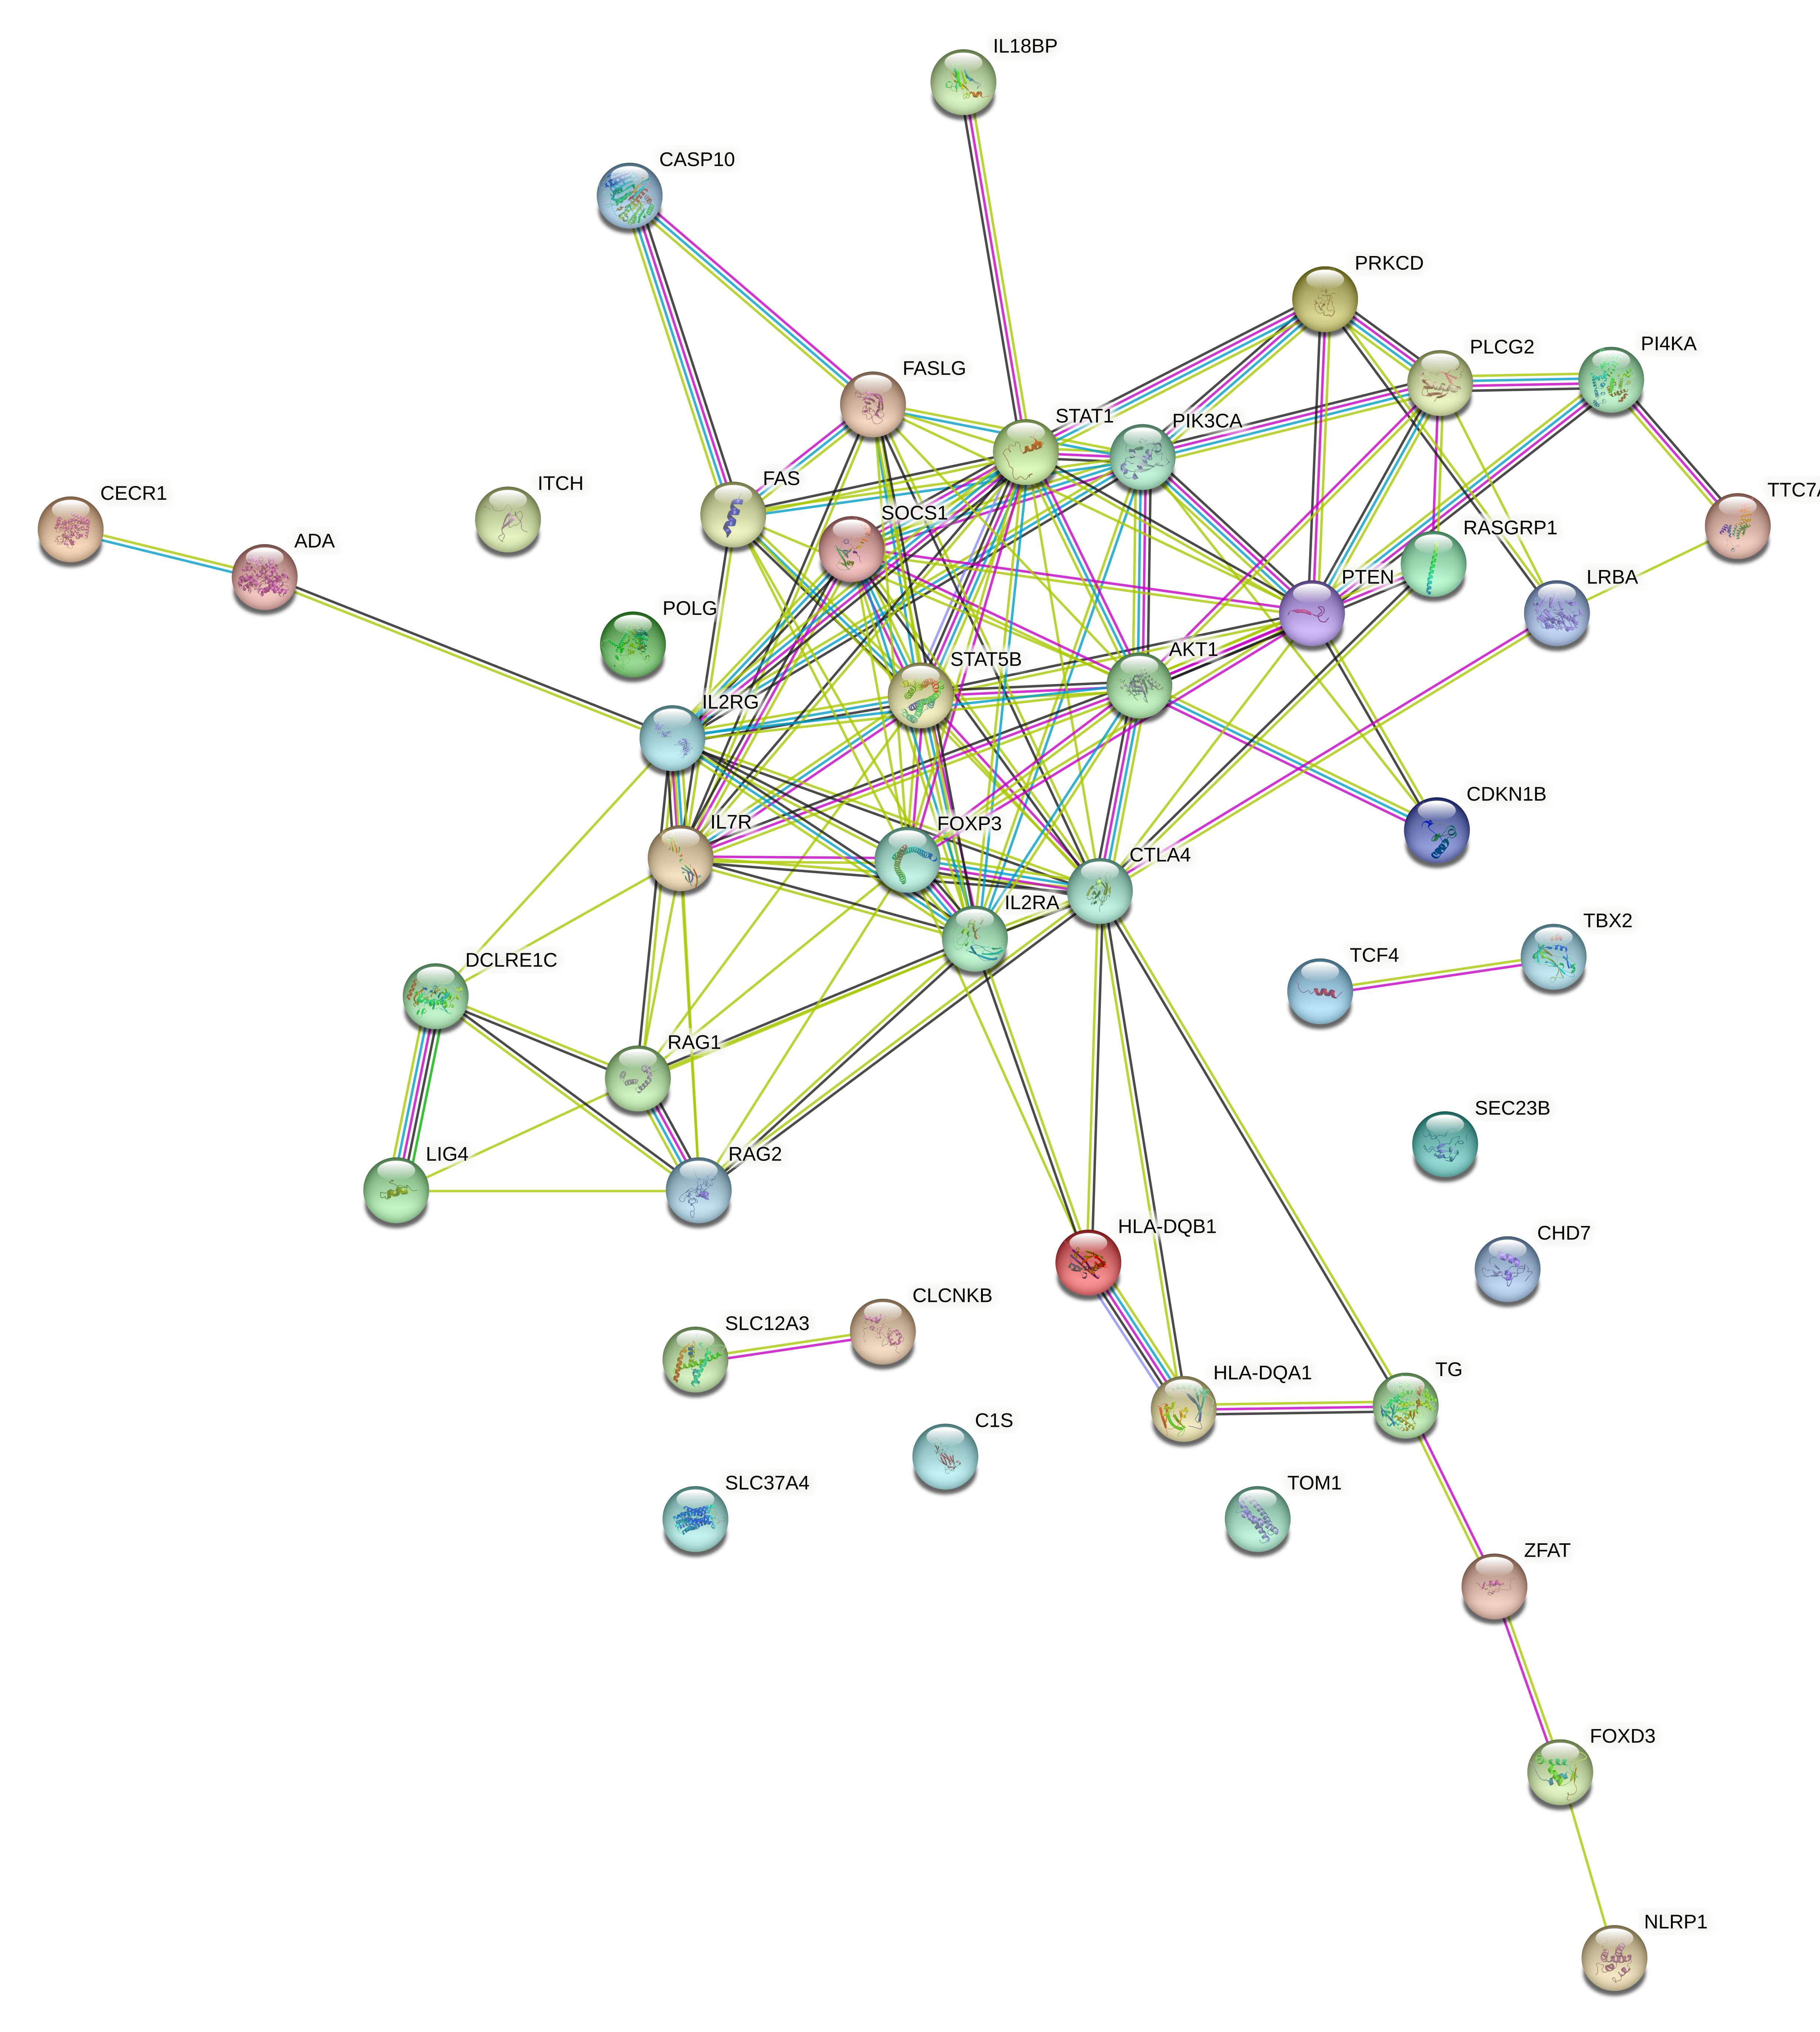
\includegraphics[scale=0.3]{figures/string_thyroiditis.png}
    
    Figure 3.1. Red de Genes HP:0100646
\end{center}


\begin{center}
 
    \includegraphics[scale=0.4]{figures/string_hashimoto.png}
    
    Figure 3.2. Red de Genes HP:000087
\end{center}

\subsection*{Comunidades}
Obtuvimos finalmente los clusters presentes en la red de genes de ambos fenotipos. Los 21 clusters que han sido obtenidos para el fenotipo de tiroiditis se muestran en la figura 3.3.

Los 5 obtenidos para Hashimoto en la figura 3.4.

\begin{center}
 
    \includegraphics[scale=0.5]{figures/comunidades_tiroiditis.png}
    
    Figure 3.3. Dendograma Tiroiditis
\end{center}

\begin{center}
 
    \includegraphics[scale=0.5]{figures/comunidades_hashimoto.png}
    
    Figure 3.4. Dendograma Hashimoto
\end{center}

\subsection*{Análisis Funcional}
Se realizó un análisis funcional (con la terminología KEGG) para identificar en que pathways biológicos intervienen todos los clusters de ambos fenotipos.

\subsection*{Comparación de clusters}
Finalmente, a partir de los pathways comunes obtenidos tras el análisis funcional, hemos determinado los clusters de cada uno de los fenotipos que están implicados en dichos procesos. Estos procesos que hemos obtenido son 'la vía de señalización JAK-STAT' y 'la enfermedad de Alzheimer'. En el primero participan el cluster 2 de Hashimoto y el 11 de Tiroitidis. En el segundo pathway participan el cluster 5 de Hashimoto y el 1 de Tiroiditis.
	\section{Discusión}
A raíz de los resultados obtenidos en la comparación de clusters, se ha determinado que hay 3 pathways donde clusters de ambos fenotipos participan: 'JAK-STAT signaling pathway', 'Alzheimer disease' y 'Bacterial invasion of epithelial cells'.Los clusters asociados a cada fenotipo en los pathways 'Bacterial invasion of epithelial cells' y 'Alzheimer disease' son los mismos. No osbtante, el gene ratio asociado al pathway 'Alzheimer disease' (0.1347), es mayor que el asociado a 'Bacterial invasion of epithelial cells' (0.1088). Por esto último descartaremos para el análisis el pathway 'Bacterial invasion of epithelial cells'.
\\ \\
Para el primer pathway los genes 'IL2RG' y 'JAK3' están presentes en el cluster de Hashimoto, así como en el de Tiroiditis. No obstante, unicamente "IL2RG" pertenece al conjunto de genes semilla. Para el segundo pathway solo encontramos un gen que esté en ambos fenotipos, el 'PIK3R2', el cual pertenece a los genes obtenidos a partir de la propagación de red. Se añade que, además, hay indicidios de  interacción física entre los genes 'IL2RG', 'JAK3' y 'PIK3R2' (R-HSA-1295544). Además dichos genes están asociados a la producción de IL-4, citoquina involucrada en procesos de regulación inmunitaria\cite{Gadani2012}. 
\\ \\
Uno de los objetivos del proyecto, y a modo de líneas futuras, era intentar expandir la red de genes de Hashimoto a partir de genes pertenecientes a la de Tiroiditis. Anteriormente hemos explicado que existen 3 genes que se encuentran en clusters de ambos fenotipos. Pero para este caso, nos interesan aquellos que están presentes en Tiroiditis pero no en Hashimoto. Unos posibles candidatos serían, basándonos en el pathway de 'vía de señalización JAK-STAT' , los genes 'IL2RB', 'EPOR','IL10RA', 'PDGFRA','PDGFRB','IL12RB2','IL27RA','IFNAR1','IL22RA1',
'EGFR','IL10RB','IFNGR2' y 'IL7R'. Basándonos en el segundo patwhay 'Alzheimer disease', encontramos los siguientes genes candidatos: 'PI4KA', 'PIK3R3' y 'PIK3R1'.
\\ \\
Recalcar que todos estos genes son candidatos y sería necesario un análisis posterior para poder determinar más relaciones de estos genes con los ya presentes en la red de genes de Hashimoto.


	\section{Conclusiones}
Tras una comparación de las redes genéticas de Tiroiditis y Hashimoto, finalmente hemos obtenido varios genes candidatos para la expansión de la red de Hashimoto.
El análisis bioinformático realizado ha consistido en varios pasos.El primero fue una expansión de ambas redes hasta obtener 200 genes en total. El siguiente paso fue la agrupación de estos genes en comunidades para su posterior análisis funcional.
Una vez las comunidades estaban asociadas a un pathway biológico, el paso final fue comparar (para ambos fenotipos) que pathways comunes compartían y, a partir de las comunidades asociadas a estos, poder determinar genes pertenecientes a la red de Tiroiditis que pudieran formar parte de la de Hashimoto.

Con estos genes candidatos se pueden realizar análisis posteriores y una investigación biológica más exhaustiva para poder decidir si realmente pueden formar parte de la red de Hashimoto.

A parte de determinar varios genes candidatos  hemos obtenido otros resultados interesantes. Por ejemplo, una relación de la tiroiditis con la enfermedad de Alzheimer. 





	
	
	%%%%%%%%%%%%%%%%%%%%%%%%%%%%%%%%%%%%%%%%%%%%%%
	%% OTRA INFORMACIÓN                         %%
	%%%%%%%%%%%%%%%%%%%%%%%%%%%%%%%%%%%%%%%%%%%%%%
	
	\begin{backmatter}
	
		\section*{Abreviaciones}%% if any
			HT: Enfermedad de Hashimoto
		
		\section*{Disponibilidad de datos y materiales}%% if any
			https://github.com/GitHubAlejandroDR/project-systems-biology
		
		\section*{Contribución de los autores}
			Usando las iniciales que habéis definido al comienzo del documento, debeis indicar la contribución al proyecto en el estilo:
			J.E : Encargado del análisis de coexpresión con R, escritura de resultados; J.R.S : modelado de red con python y automatizado del código, escritura de métodos; ...
			OJO: que sea realista con los registros que hay en vuestros repositorios de github. 
		
		
		%%%%%%%%%%%%%%%%%%%%%%%%%%%%%%%%%%%%%%%%%%%%%%%%%%%%%%%%%%%%%%%%%%%%%%%%%%%%%%%%%%%%%%%%
		%% BIBLIOGRAFIA: no teneis que tocar nada, solo sustituir el archivo bibliography.bib %%
		%% por el que hayais generado vosotros                                                %%
		%%%%%%%%%%%%%%%%%%%%%%%%%%%%%%%%%%%%%%%%%%%%%%%%%%%%%%%%%%%%%%%%%%%%%%%%%%%%%%%%%%%%%%%%
		
		\bibliographystyle{bmc-mathphys} % Style BST file (bmc-mathphys, vancouver, spbasic).
		\bibliography{bibliography}      % Bibliography file (usually '*.bib' )
	
	\end{backmatter}
\end{document}
